% =====================================================================
%  English edition of reports/bao_cao_fusion.tex. The Vietnamese file is
%  kept unchanged as the reported version; the two are meant to stay in
%  step, so a change to one belongs in the other as well.
%
%  Compile with pdfLaTeX (Overleaf's default) -- nothing to configure.
%  To use system fonts instead, switch the compiler to XeLaTeX and replace
%  the inputenc/fontenc/lmodern lines below with:
%      \usepackage{fontspec}
%      \setmainfont{TeX Gyre Termes}
% =====================================================================
\documentclass[11pt,a4paper]{article}

\usepackage[utf8]{inputenc}
% The body is English, for which [T1] would be correct. [T5] is kept for one
% reason only: the author name carries Vietnamese diacritics that T1 cannot
% render. T5 covers the full ASCII range, so English text sets identically.
\usepackage[T5]{fontenc}
\usepackage{lmodern}

\usepackage[margin=2.6cm]{geometry}
\usepackage{amsmath}
\usepackage{amssymb}
\usepackage{booktabs}
\usepackage{array}
\usepackage{caption}
\usepackage{microtype}
\usepackage{enumitem}
\usepackage{float}
\usepackage{tikz}
\usetikzlibrary{arrows.meta, positioning}
\usepackage[hidelinks]{hyperref}

% No \renewcommand block for captions here: article already labels
% everything in English.

\captionsetup[table]{skip=6pt}
\captionsetup[figure]{skip=8pt}
\newcolumntype{R}{>{\raggedleft\arraybackslash}p{2.7cm}}

\title{\bfseries Two-Stage Fusion for HRM-PET:\\
multi-source routing and gated auxiliary classification}
\author{Nguyễn Thiên Trường}
\date{August 2026}

\begin{document}
\maketitle

\begin{abstract}
We replace the single-source router of HRM-PET with a fusion of two evidence
sources, then use that second source as an auxiliary classifier whose weight is
controlled by a per-sample gate. The second source is a second-order
random-projection classification head in the style of RanPAC, built directly on
the LoRA features HRM-PET has already trained. The method therefore trains no
additional parameters and still respects the exemplar-free protocol. Across
three continual-learning benchmarks and four seeds, routing accuracy rises by
$+1.10$ to $+2.26$ points and classification accuracy by $+0.69$ to $+1.50$
points; on both axes the gain is several times the seed-to-seed standard
deviation. The two retention metrics show no change distinguishable from zero,
and we claim no improvement there. The gain survives on five ViT-B/16
backbones differing in pretraining: the baseline spans $5.6$ points while
the gain spans $0.9$. The added compute is exactly one forward pass
per sample.
\end{abstract}

\tableofcontents
\bigskip

\section{Introduction}

\subsection{The HRM-PET Pipeline}

HRM-PET processes every input sample in four steps:

\begin{enumerate}[leftmargin=*, itemsep=2pt]
\item \textbf{Task-identity inference} (TII): estimate which task the sample
      belongs to, based on prompt energy.
\item \textbf{Routing}: send the sample to the frozen LoRA parameter set of the
      task selected in step 1.
\item \textbf{Refinement}: two mechanisms, DRM and CRM, revise the routing
      decision.
\item \textbf{Classification}: a head shared across all tasks issues the final
      prediction.
\end{enumerate}

The quality of this entire chain rests on a single routing signal, produced at
step 1.

\begin{figure}[H]
\centering
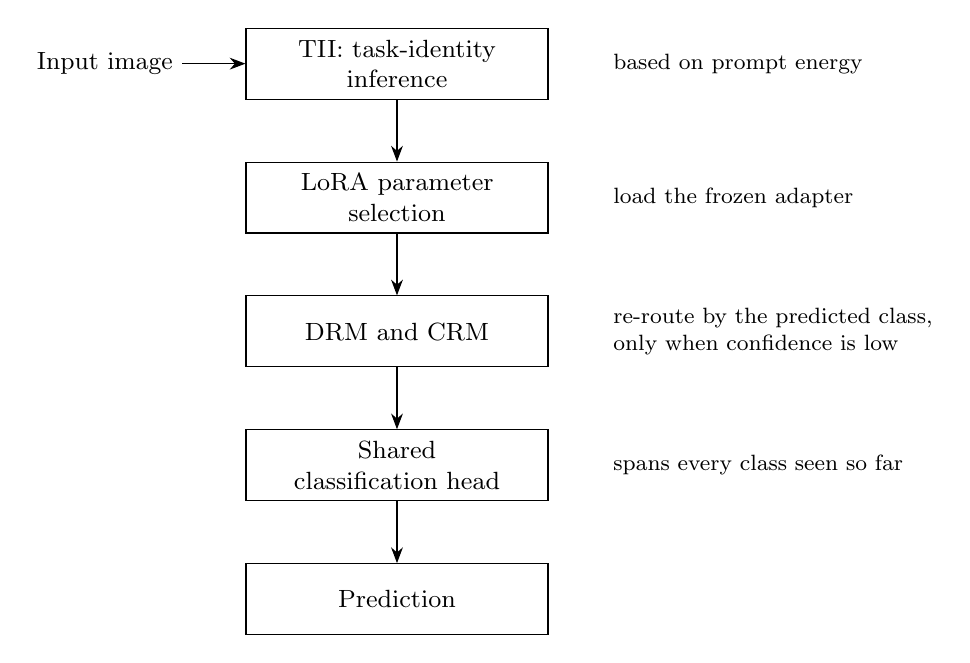
\begin{tikzpicture}[
  font=\small, >={Stealth[length=2mm]},
  box/.style={draw, minimum height=9mm, text width=3.6cm, align=center},
  lbl/.style={font=\footnotesize, align=left}
]
% Explicit breaks: at text width=3.6cm the English labels would otherwise be
% hyphenated mid-word inside the boxes ("LoRA parame-ter", "Shared classi-
% fication"), which reads badly in a diagram. Each line below fits the width.
\node[box] (tii) at (0,0)    {TII: task-identity\\inference};
\node[box] (lo)  at (0,-1.7) {LoRA parameter\\selection};
\node[box] (drm) at (0,-3.4) {DRM and CRM};
\node[box] (cl)  at (0,-5.1) {Shared\\classification head};
\node[box] (out) at (0,-6.8) {Prediction};

\draw[->] (tii) -- (lo);
\draw[->] (lo)  -- (drm);
\draw[->] (drm) -- (cl);
\draw[->] (cl)  -- (out);

\node[lbl, right=7mm of tii] {based on prompt energy};
\node[lbl, right=7mm of lo]  {load the frozen adapter};
\node[lbl, right=7mm of drm] {re-route by the predicted class,\\only when confidence is low};
\node[lbl, right=7mm of cl]  {spans every class seen so far};

\node[left=8mm of tii] (in) {Input image};
\draw[->] (in) -- (tii);
\end{tikzpicture}
\caption{The original HRM-PET pipeline. The whole chain depends on a single
routing signal, produced in the first block. The last block is the shared
classification head; that property is the cause of the second limitation
analysed in Sect.~\ref{sec:analysis}.}
\label{fig:hrmpet}
\end{figure}

\subsection{Two Limitations}

This report identifies two limitations of the design above. First, the TII
signal is not the best routing signal that can be extracted from the trained
model itself. Second, even when routing improves, most of that improvement does
not convert into classification accuracy, for a reason that lies in the
architecture rather than in routing quality. Section~\ref{sec:analysis} presents
the measurements for both.

\subsection{Contributions}

Table~\ref{tab:routing} shows the headroom that remains. On ImageNet-R the TII
signal routes $63.80\,\%$ of samples correctly; after HRM-PET's two refinement
steps, DRM and CRM, that figure reaches $77.79\,\%$. A random-projection
classification head, training no additional parameters, reaches $77.12\,\%$ on
its own --- on a par with that entire refinement procedure. More importantly, it
routes correctly $19.2\,\%$ of the samples that TII gets wrong, so the union of
the two sources reaches $82.99\,\%$. A similar gap recurs on CIFAR-100 ($89.82$
versus $92.86$) and CUB-200 ($93.21$ versus $96.26$). In other words, HRM-PET
makes its routing decision from a single source of evidence, while a second
source already sits inside the trained model.

We therefore propose two fusion stages, both placed at inference time. The first
blends the task-level scores of TII with those of the random-projection head
after standardising the two sources onto a common scale, then hands the result
to DRM and CRM as a better starting point. The second stage addresses a
different limitation: better routing does not automatically become better
classification, because the shared head frequently predicts the correct class in
spite of a wrong routing decision, so fixing the routing of those samples
changes nothing. This stage uses the random-projection head itself as a
secondary classifier, weighted per sample in inverse proportion to how decided
the primary classifier already is, so that the blend opens only on contested
samples --- the only place where it can change a prediction.
Figure~\ref{fig:pipeline} shows where both stages sit in the pipeline.

In summary, this report contributes three things. \emph{First}, we propose
fusion at the routing level, combining TII with a training-free classification
head to raise routing accuracy in PET-based methods
(Sect.~\ref{sec:stage1}). \emph{Second}, we propose fusion at the
classification level with a margin-based gate, using that same head as the
second source and intervening only on samples the primary head is still
undecided about (Sect.~\ref{sec:stage2}). \emph{Third}, we validate the effect
on three continual-learning benchmarks and four seeds, at an added cost of
exactly one forward pass per sample and with no additional parameters trained.

\begin{figure}[H]
\centering
\resizebox{\textwidth}{!}{%
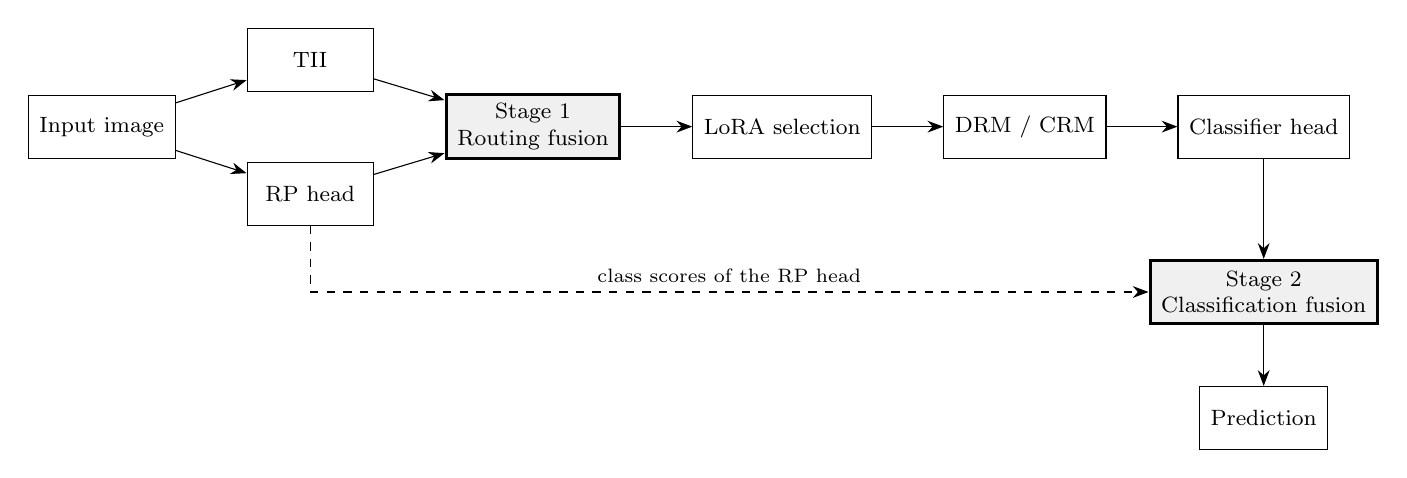
\begin{tikzpicture}[
  font=\footnotesize,
  >={Stealth[length=2mm]},
  box/.style={draw, minimum height=8mm, minimum width=1.6cm, inner xsep=4pt, align=center},
  hl/.style={box, very thick, fill=black!6}
]
% Each box is chained off the previous one's east edge, so what is specified is
% the GAP and the width is free to be whatever the label needs. Fixed centre
% coordinates cannot work here: box width depends on label length, so longer
% words silently eat the gap. With the old centres the LoRA-to-DRM gap fell to
% 1.49pt against a 2mm (5.69pt) arrow tip, i.e. the arrowhead was drawn inside
% the neighbouring box. 9mm keeps every gap at 25.61pt in both languages.
\node[box] (in) at (0, 0) {Input image};
\coordinate (up) at (0, 0.85);
\coordinate (dn) at (0,-0.85);
\coordinate (r1) at ([xshift=9mm]in.east);
\node[box, anchor=west] (tii) at (r1 |- up) {TII};
\node[box, anchor=west] (rp)  at (r1 |- dn) {RP head};
% anchored on rp, not tii: rp carries the longer label of the two, so it is the
% binding constraint if either label is ever edited.
\coordinate (r2) at ([xshift=9mm]rp.east);
\node[hl,  anchor=west] (f1) at (r2 |- in) {Stage 1\\Routing fusion};
\node[box, anchor=west] (lo) at ([xshift=9mm]f1.east) {LoRA selection};
\node[box, anchor=west] (dr) at ([xshift=9mm]lo.east) {DRM / CRM};
\node[box, anchor=west] (cl) at ([xshift=9mm]dr.east) {Classifier head};
\node[hl]  (f2) at ([yshift=-2.1cm]cl.center) {Stage 2\\Classification fusion};
\node[box] (out) at ([yshift=-3.7cm]cl.center) {Prediction};

\draw[->] (in) -- (tii);
\draw[->] (in) -- (rp);
\draw[->] (tii) -- (f1);
\draw[->] (rp) -- (f1);
\draw[->] (f1) -- (lo);
\draw[->] (lo) -- (dr);
\draw[->] (dr) -- (cl);
\draw[->] (cl) -- (f2);
\draw[->] (f2) -- (out);
\draw[->, dashed] (rp.south) |- node[pos=0.75, above, font=\scriptsize]
      {class scores of the RP head} (f2.west);
\end{tikzpicture}}
\caption{The inference pipeline. The bold-outlined blocks are the two added
components. The RP head is computed exactly once and supplies both stages: task
scores for the first, class scores for the second (dashed line).}
\label{fig:pipeline}
\end{figure}

\section{Analysis of the Two Limitations}
\label{sec:analysis}

\subsection{First Limitation: the Routing Signal Is Not Optimal}

We build a random-projection classification head (RP head for short) on
HRM-PET's own LoRA features. The RP head gives higher routing accuracy than TII
on all three benchmarks. More importantly, the \emph{union} of the two routers
is far above what HRM-PET achieves after refinement by DRM and CRM.

\begin{table}[htbp]
\centering
\caption{Routing accuracy (\%), seed 42. The last row is the fraction of samples
on which at least one of the two routers is correct, that is, the upper bound
attainable by combining the two sources.}
\label{tab:routing}
\begin{tabular}{lrrr}
\toprule
Routing source & ImageNet-R & CIFAR-100 & CUB-200 \\
\midrule
TII                        & 63.80 & 81.21 & 92.96 \\
HRM-PET after DRM and CRM  & 77.79 & 89.82 & 93.21 \\
RP head                    & 77.12 & 89.51 & 94.02 \\
\midrule
Union of TII and RP head   & \textbf{82.99} & \textbf{92.86} & \textbf{96.26} \\
\bottomrule
\end{tabular}
\end{table}

The two routers fail on different sets of samples. On ImageNet-R, the RP head
routes correctly $19.2\,\%$ of the samples TII routes incorrectly. This
complementarity is the necessary condition for fusion to mean anything: if both
sources failed on the same samples, their union would not exceed the stronger
source.

\subsection{Second Limitation: Better Routing Is Not Better Classification}

Once the routing stage improves, a second phenomenon appears: the gain in
routing accuracy converts into classification accuracy at a rate of only
$14$--$21\,\%$, and on CUB-200 it does not convert at all.

The cause is architectural. The shared classification head spans \emph{all}
classes seen so far, so a misrouted sample is still frequently classified
correctly. In that case, fixing the routing path brings no benefit; conversely,
re-routing a sample that was already classified correctly can turn the result
wrong.

The RP head, however, is not merely a router. It is a complete classifier in its
own right, one the routing stage ignored. Table~\ref{tab:cls} measures the
complementarity between the two classifiers.

\begin{table}[htbp]
\centering
\caption{Complementarity at the classification level (\%), seed 42. The last
column is the fraction of samples the routed classifier gets wrong and the RP
head gets right.}
\label{tab:cls}
\begin{tabular}{lrrrr}
\toprule
Dataset & Routed head & RP head & Union & RP head's contribution \\
\midrule
ImageNet-R & 74.31 & 70.08 & 78.89 & $+4.58$ \\
CIFAR-100  & 89.97 & 88.76 & 92.40 & $+2.43$ \\
CUB-200    & 86.48 & 87.50 & 90.35 & $+3.87$ \\
\bottomrule
\end{tabular}
\end{table}

Even on ImageNet-R, where the RP head's overall accuracy is $4$ points lower, it
still classifies correctly $4.58\,\%$ of the samples the primary head cannot
handle.

\section{Proposed Method}

\subsection{The Second Source of Evidence}

\subsubsection{The Idea}

The underlying idea is to expand the representation space before classifying
linearly. In the $768$-dimensional feature space the classes overlap to the
point that no hyperplane separates them. After projecting into a
$10^4$-dimensional space and applying a nonlinearity, the classes have room to
separate, and a linear classifier in the new space becomes expressive enough.

The projection matrix is entirely random and is never trained. This is not a
trade-off but a necessary condition: any parameter updated by gradients across a
task sequence can be overwritten by a later task, whereas a frozen matrix drawn
from a fixed seed never changes and need not even be stored. Eliminating
trainable parameters altogether is the premise for the order-invariance property
presented in Sect.~\ref{sec:order}.

The second source consists of a frozen random projection, regenerable from a
fixed seed, followed by a ReLU nonlinearity and a ridge-regression solve on an
accumulated Gram matrix. No parameter is trained. The feature $f$ is extracted
from \emph{one} fixed LoRA parameter set of HRM-PET, which serves as
first-session adaptation:
\begin{align}
h &= \mathrm{ReLU}(f W), \qquad W \text{ frozen, regenerable from a seed},\\
G &= \sum_n h_n h_n^{\top}, \qquad
C = \sum_n h_n\,\mathrm{onehot}(y_n)^{\top},\\
s &= h^{\top} (G + \lambda I)^{-1} C .
\label{eq:rp}
\end{align}

The system stores only the two aggregate quantities $G$ and $C$; the projection
matrix $W$ is regenerated from its seed. No per-sample feature and no image from
a previous task is retained, so the exemplar-free protocol is preserved.

\begin{table}[H]
\centering
\caption{Notation for the three equations above. Sizes follow the configuration
used in this report: $L = 768$ is the feature dimension, $M = 10^4$ the
projected dimension, $K$ the number of classes seen so far, and $n$ the index
running over training samples.}
\label{tab:notation}
\begin{tabular}{@{}llp{7.4cm}@{}}
\toprule
Symbol & Size & Meaning \\
\midrule
$f$        & $L$          & image feature, extracted from one fixed LoRA parameter set \\
$W$        & $L \times M$ & random projection matrix, frozen, regenerable from a seed \\
$h$        & $M$          & representation after projection and ReLU \\
$y_n$      & ---          & label of the $n$-th sample \\
$G$        & $M \times M$ & Gram matrix, accumulated over every sample seen \\
$C$        & $M \times K$ & correlation matrix between representation dimensions and classes \\
$\lambda$  & scalar       & ridge regularisation coefficient \\
$I$        & $M \times M$ & identity matrix \\
$s$        & $K$          & per-class scores, the output of the second source \\
\bottomrule
\end{tabular}
\end{table}

The three equations correspond to three steps. The first projects the feature
into $M$ dimensions and applies the nonlinearity. The second accumulates two
second-order statistics: $G$ records co-occurrence between representation
dimensions, $C$ records the association between representation dimensions and
classes. Both are updated as each task is learned and never require re-reading
old data. The third solves the ridge regression, giving the weight matrix
$W_o = (G + \lambda I)^{-1} C$ and the scores $s = h^{\top} W_o$; this step is
performed once at the end of each task.

\subsubsection{Why the Nonlinearity Is Mandatory}

If ReLU is removed from \eqref{eq:rp}, the map $h = fW$ becomes linear. Then,
however many of the $10^4$ dimensions $h$ has, its span is a subspace of
dimension at most the rank of $W$, that is $768$. Ridge regression on $h$ is then
mathematically equivalent to ridge regression on $f$, and the projection
contributes nothing but memory cost. It is exactly the clipping performed by
ReLU that takes the representation out of that subspace and creates genuinely
new feature dimensions.

\subsubsection{The Role of the Gram Inverse}

Using $C$ alone and dropping $(G + \lambda I)^{-1}$ reduces the model to a
class-prototype classifier. That is ineffective on ViT features because a few
high-energy directions occur in every class, making the prototypes strongly
correlated with one another and drowning out the discriminative component. The
Gram inverse performs whitening: directions that are common, and therefore large
in $G$, are down-weighted, leaving the directions that genuinely separate
classes.

The experiments support this argument: a variant that re-scores using
Mahalanobis distance in the original $768$-dimensional space, with both
per-class and shared covariance, gives routing accuracy $84.3$ against the
baseline's $93.21$ on CUB-200.

\subsubsection{Order Invariance and Its Consequence for Forgetting}
\label{sec:order}

Both $G$ and $C$ are sums accumulated over samples, and addition commutes.
Hence
\begin{equation}
G = \sum_{t=1}^{T} G_t
\end{equation}
does not depend on the order of the tasks, and the solution after the last task
coincides with the one obtained by training linearly on all the data at once.
The second source therefore \emph{cannot} forget in the sense of catastrophic
forgetting: this is an algebraic property, not an experimental result.

\subsubsection{The Constraint on the Feature Extractor}
\label{sec:fixed-extractor}

The feature $f$ must come from an extractor that is \emph{fixed for the whole
task sequence}. There are two independent reasons.

First, $G$ and $C$ are accumulated across all tasks. Addition is meaningful only
when the terms live in the same feature space. If each task used a different
LoRA parameter set, the vectors $h$ would belong to incompatible spaces and the
Gram matrix would be meaningless. The ReLU makes the problem worse: the same
image passed through two different adapters activates two different sets of
dimensions, which is a discrete change in the structure of the vector rather
than a small, uniform perturbation.

Second, a causality constraint. The statistics of the first task must be
accumulated at the moment that task is learned, because the exemplar-free
protocol forbids revisiting old data. At that moment, the LoRA parameter sets of
all later tasks do not yet exist.

The two constraints together leave only two options: the unadapted backbone, or
the LoRA parameter set of the first task. We choose the second;
Sect.~\ref{sec:closed} gives the measurements comparing the two.

\subsubsection{Contrast with TII}
\begin{table}[htbp]
\centering
\caption{The two routers side by side. The two sources exploit two different
kinds of evidence about the same question, which is the basis for expecting them
to fail on different sets of samples.}
\label{tab:tii-vs-rp}
\begin{tabular}{@{}p{3.3cm}p{4.9cm}p{5.2cm}@{}}
\toprule
 & TII & RP head \\
\midrule
Evidence used
  & the per-task prompts
  & the $768$-dimensional image feature \\
Quantity measured
  & the model's uncertainty when each prompt set is attached
  & the similarity between the feature and the class prototypes \\
How parameters are obtained
  & backpropagation over many epochs
  & closed-form, single step \\
Trainable parameters
  & yes
  & no \\
Affected by forgetting
  & yes
  & no, by order invariance \\
Acc@task, ImageNet-R
  & $63.80$
  & $77.12$ \\
\bottomrule
\end{tabular}
\end{table}

The essential difference is in the second row: TII assesses how confident the
model is when each prompt set is attached, whereas the RP head assesses how
similar the sample's feature is to each class prototype. The two criteria differ
in kind, so there is no reason for them to fail on the same samples.

\subsection{First Stage: Fusion at the Routing Level}
\label{sec:stage1}

\subsubsection{Converting Class Scores into Task Scores}

Both sources emit scores over \emph{classes}. For routing, a task's score is
taken as the maximum over the classes belonging to it:
\begin{equation}
\ell^{\mathrm{task}}_t = \max_{c \,\in\, \mathcal{C}_t} \ell_c ,
\qquad
s^{\mathrm{task}}_t = \max_{c \,\in\, \mathcal{C}_t} s_c ,
\label{eq:taskscore}
\end{equation}
where $\mathcal{C}_t$ is the class set of task $t$, $\ell$ the per-class logits
of TII and $s$ the per-class scores of the RP head. The same reduction is applied
to both sources; the two resulting vectors are exactly the
$\ell^{\mathrm{TII}}$ and $s^{\mathrm{RP}}$ appearing in \eqref{eq:route}. The
maximum matches the question being asked --- \emph{does this task contain the
correct class} --- whereas a sum or a mean would favour tasks with many classes
at middling similarity over one class at high similarity.

\subsubsection{Fusion and Standardisation}

Let $z(\cdot)$ denote standardisation to zero mean and unit variance, computed
separately for each sample over the tasks seen so far. The task scores of the
two sources are combined linearly; the highest-scoring task is selected, and this
routing decision is passed into HRM-PET's existing DRM, CRM and classification
head:
\begin{equation}
\mathrm{fused} = w\, z(\ell^{\mathrm{TII}}) + (1-w)\, z(s^{\mathrm{RP}}),
\qquad w = 0.7 .
\label{eq:route}
\end{equation}

The standardisation here is mandatory. The TII logits are dispersed over a range
orders of magnitude wider than the ridge-regression scores. Combined directly,
TII dominates at every weight, and routing accuracy falls \emph{below} that of
the RP head alone: $68.24$ against $77.12$. A fused result below both of its
components is the characteristic signature of a scale mismatch.

\subsubsection{Choosing the Fusion Weight}
\label{sec:choose-w}

The weight $w$ sits on TII, so $w = 1.0$ corresponds to the baseline. The value
$w = 0.7$ was chosen by the criterion \emph{every metric improves on every
seed}, not by maximising mean Acc@1.

\begin{table}[htbp]
\centering
\caption{Basis for choosing $w$, measured on ImageNet-R over four seeds, at the
stage where only routing fusion was present.}
\label{tab:choose-w}
\begin{tabular}{@{}p{5.4cm}p{4.6cm}p{2.6cm}@{}}
\toprule
 & $w = 0.6$ & $w = 0.7$ \\
\midrule
Mean Acc@1 & $+0.48$ & $+0.31$ \\
All six metrics improve on every seed
  & no (Forgetting and Backward degrade on seed 43) & yes \\
\bottomrule
\end{tabular}
\end{table}

The configuration $w = 0.6$ gives a larger mean Acc@1 gain but is not stable
across seeds. We prioritise consistency, since a method with a higher average
gain that occasionally degrades a retention metric is hard to regard as a
reliable improvement.

\subsubsection{Sweeping the Two Weights Jointly}

The two weights were chosen one after the other: $w$ was fixed before the second
stage existed, $\beta$ afterwards. Since both act on the same decision, this
raises the question of whether the second stage took over part of the first
stage's work and moved the optimum for $w$. Table~\ref{tab:joint} answers it
with a full grid.

\begin{table}[htbp]
\centering
\caption{Acc@1 over the $w \times \beta$ grid, ImageNet-R seed 42, full system
with the margin gate. The bold cell is the configuration in use.}
\label{tab:joint}
\begin{tabular}{@{}lrrr@{}}
\toprule
 & $\beta = 0.3$ & $\beta = 0.5$ & $\beta = 0.7$ \\
\midrule
$w = 0.6$ & 75.28 & 75.61 & 75.29 \\
$w = 0.7$ & 75.22 & \textbf{75.51} & 75.24 \\
$w = 0.8$ & 75.12 & 75.50 & 75.27 \\
\bottomrule
\end{tabular}
\end{table}

\textbf{The two weights barely interact.} $\beta = 0.5$ is the best value at
\emph{all three} settings of $w$, and its two neighbours lose by roughly the same
amount in every row. Tuning them sequentially therefore cost nothing --- which is
now a measurement rather than an assumption.

\textbf{Acc@1 is nearly flat in $w$; Acc@task is not.} At $\beta = 0.5$ the three
values of $w$ span $0.11$ points of Acc@1 while Acc@task spans $1.01$ ($80.39$,
$79.97$, $79.37$). Lowering $w$ buys routing accuracy of which only about
one ninth converts into Acc@1 --- exactly the phenomenon analysed in
Sect.~\ref{sec:analysis}, now measured along a continuous axis.

\textbf{On choosing between $0.6$ and $0.7$.} The original criterion --- every
metric improving on every seed --- is the one Sect.~\ref{sec:limits} itself
identifies as circular, so we no longer invoke it. By mean Acc@1 over four seeds
$w = 0.6$ leads by $0.17$ points, and in the grid above by $0.10$; both are
smaller than the $0.416$ standard deviation of the Acc@1 change itself across
seeds. The two values are therefore \emph{not resolvable} with the data we have.
We keep $w = 0.7$ because it is the value every number in this report was
measured with, and say so rather than defending it with the old criterion.

\subsection{Second Stage: Gated Fusion at the Classification Level}
\label{sec:stage2}

The first version combined the two classifiers with a weight $\beta$ fixed for
every sample. That produced a systematic regression: the cross-entropy loss on
CIFAR-100 rose by $+0.019 \pm 0.003$, even though accuracy still improved.

The cause is that a fixed weight treats two fundamentally different kinds of
sample identically: one where the primary classifier predicts with probability
$p = 0.97$, and one where it has not settled between classes. On CIFAR-100 the
first kind is the large majority. Spending $30\,\%$ of the decision on the second
source for exactly those samples only flattens the probability distribution at a
prediction that was already correct: cross-entropy rises immediately, while the
$\arg\max$ does not change.

The remedy is to let $\beta$ vary per sample, in inverse proportion to how
decided the primary classifier is. The quantity used to measure decidedness is
the margin between its own two highest-scoring classes. The reasoning behind
this choice: fusion can change a prediction only by displacing the top-ranked
class, and the most plausible replacement is the runner-up. Writing $p_{(1)}$
and $p_{(2)}$ for the two largest probabilities of the routed classifier:
\begin{equation}
\beta_i = \beta \left( 1 - \frac{p_{(1)} - p_{(2)}}{p_{(1)} + p_{(2)}} \right),
\qquad \beta = 0.5 .
\label{eq:gate}
\end{equation}

The margin is normalised by the sum of the two largest probabilities rather than
by $1$. Setting $r = p_{(2)}/p_{(1)}$, the bracketed expression becomes
$1 - (1-r)/(1+r)$, that is, it \emph{depends only on the ratio between the two
leading classes} and is independent of the probability mass they hold together.
This is the desired property: how threatening the runner-up is should be
measured by its relative standing, not by its absolute value.

The final scores are combined and then returned to the scale of the original
logits:
\begin{align}
m_i &= (1 - \beta_i)\, z(\ell_i) + \beta_i\, z(s_i),\\
\hat{\ell}_i &= m_i \cdot \mathrm{std}(\ell_i) + \mathrm{mean}(\ell_i).
\label{eq:affine}
\end{align}

\begin{table}[htbp]
\centering
\caption{Effective gate weights under \eqref{eq:gate} with $\beta = 0.5$.}
\label{tab:gate-example}
\begin{tabular}{@{}lrrrr@{}}
\toprule
State of the primary classifier & $p_{(1)}$ & $p_{(2)}$ & Margin & $\beta_i$ \\
\midrule
Very decided       & 0.97 & 0.01 & 0.980 & 0.010 \\
Decided            & 0.90 & 0.02 & 0.957 & 0.022 \\
Undecided          & 0.35 & 0.30 & 0.077 & 0.462 \\
\bottomrule
\end{tabular}
\end{table}

Table~\ref{tab:gate-example} shows the mechanism behaving as designed: on
confidently predicted samples the second source retains only about $2\,\%$ of the
decision; on undecided samples that share rises to $46\,\%$. The gate introduces
no additional hyperparameter and applies a single rule across all three
benchmarks.

The transform \eqref{eq:affine} is a per-sample affine map with a positive
multiplier, hence monotonically increasing: the ranking among classes is
preserved and every accuracy metric is unchanged. Its only role is to bring the
scale of the logits back to a level comparable with the baseline when computing
cross-entropy. Using the moments of $\ell$ as the reference also guarantees that
at $\beta_i = 0$ the method returns exactly the original logits.

\section{Experimental Setup}

\subsection{Configuration}

The backbone is ViT-B/16 pre-trained on ImageNet-21K, adapted with LoRA of rank
$8$. Each dataset is split into a sequence of $10$ tasks and every experiment is
repeated over four seeds, $42$, $43$, $44$ and $45$. All LoRA and TII
checkpoints are retrained from scratch for each seed. Evaluation uses the same
checkpoints for both the baseline and the proposed method, so the observed
differences reflect precisely the inference-time change, uncontaminated by
training noise.

RP head hyperparameters: projection dimension $10^4$, ReLU nonlinearity,
regularisation coefficient $\lambda = 10^4$. No temperature scaling is applied.

\subsection{Metrics}

Let $a_{i,t}$ denote the accuracy on task $i$ measured at stage $t$, and $T$ the
total number of tasks.

\begin{itemize}[leftmargin=*, itemsep=2pt]
\item \textbf{Acc@task}: routing accuracy, the fraction of samples assigned to
      the correct task.
\item \textbf{Acc@1}, \textbf{Acc@5}: classification accuracy at the top-ranked
      label and within the top five.
\item \textbf{Loss}: the cross-entropy loss.
\item \textbf{Forgetting} and \textbf{Backward}: two metrics of how well the
      model retains old knowledge, computed over the full result matrix.
\end{itemize}

\begin{equation}
\mathrm{Forgetting} = \frac{1}{T}\sum_{i=1}^{T}
\Big( \max_{t} a_{i,t} - a_{i,T} \Big),
\qquad
\mathrm{Backward} = \frac{1}{T}\sum_{i=1}^{T} \big( a_{i,T} - a_{i,i} \big).
\end{equation}

For Loss and Forgetting, lower is better; for the other four metrics, higher is
better. One point deserves attention: both Forgetting and Backward compare a
task against itself at an earlier moment, not against another method. This
property is used again in Sect.~\ref{sec:ramp}.

\section{Results}
\label{sec:results}

Table~\ref{tab:main} summarises the results on all three benchmarks. Values are
means $\pm$ standard deviation over four seeds. The \emph{Change} column is
computed pairwise: the difference between the proposed method and the baseline
is taken per seed, and only then averaged. The standard deviation of that column
therefore reflects the stability of the improvement itself, unaffected by
differences in difficulty between seeds.

\begin{table}[H]
\centering
\caption{Results on three benchmarks, mean $\pm$ standard deviation over four
seeds 42, 43, 44, 45.}
\label{tab:main}
\begin{tabular}{@{}p{0.4cm}lRRR@{}}
\toprule
\multicolumn{2}{@{}l}{Dataset and metric} & HRM-PET & Proposed & Change \\
\midrule
\multicolumn{5}{l}{\emph{Split-ImageNet-R}}\\
& Acc@task   & $77.58 \pm 0.33$  & $79.85 \pm 0.18$  & $+2.264 \pm 0.158$ \\
& Acc@1      & $73.94 \pm 0.48$  & $75.18 \pm 0.24$  & $+1.236 \pm 0.416$ \\
& Acc@5      & $86.71 \pm 0.21$  & $88.02 \pm 0.17$  & $+1.312 \pm 0.148$ \\
& Loss       & $1.23 \pm 0.01$   & $1.19 \pm 0.01$   & $-0.040 \pm 0.002$ \\
& Forgetting & $3.36 \pm 0.56$   & $3.30 \pm 0.35$   & $-0.056 \pm 0.334$ \\
& Backward   & $-3.16 \pm 0.61$  & $-3.20 \pm 0.42$  & $-0.047 \pm 0.282$ \\
\addlinespace
\multicolumn{5}{l}{\emph{Split-CIFAR100}}\\
& Acc@task   & $89.77 \pm 0.11$  & $90.87 \pm 0.09$  & $+1.103 \pm 0.066$ \\
& Acc@1      & $89.78 \pm 0.03$  & $90.47 \pm 0.05$  & $+0.690 \pm 0.063$ \\
& Acc@5      & $98.65 \pm 0.03$  & $98.86 \pm 0.07$  & $+0.217 \pm 0.057$ \\
& Loss       & $0.39 \pm 0.00$   & $0.39 \pm 0.00$   & $-0.000 \pm 0.001$ \\
& Forgetting & $3.89 \pm 0.08$   & $3.74 \pm 0.12$   & $-0.156 \pm 0.098$ \\
& Backward   & $-3.87 \pm 0.07$  & $-3.73 \pm 0.11$  & $+0.142 \pm 0.097$ \\
\addlinespace
\multicolumn{5}{l}{\emph{Split-CUB200}}\\
& Acc@task   & $93.12 \pm 0.14$  & $94.34 \pm 0.10$  & $+1.226 \pm 0.149$ \\
& Acc@1      & $86.38 \pm 0.25$  & $87.88 \pm 0.27$  & $+1.495 \pm 0.353$ \\
& Acc@5      & $97.04 \pm 0.10$  & $97.44 \pm 0.13$  & $+0.400 \pm 0.103$ \\
& Loss       & $0.57 \pm 0.00$   & $0.53 \pm 0.01$   & $-0.036 \pm 0.004$ \\
& Forgetting & $2.54 \pm 0.35$   & $2.18 \pm 0.12$   & $-0.359 \pm 0.325$ \\
& Backward   & $-2.42 \pm 0.39$  & $-2.14 \pm 0.13$  & $+0.279 \pm 0.391$ \\
\bottomrule
\end{tabular}
\end{table}

The six metrics are not six independent events. They measure three axes, and
stating the result by axis says more, and withstands scrutiny better, than a
pooled count. The decisive quantity here is the ratio between the change and the
standard deviation of that change: below $2$, nothing is resolvable.

\textbf{The routing axis (Acc@task): a solid improvement.} The gain is $+1.10$
to $+2.26$ points, with that ratio between $8$ and $17$. This is the axis the
method acts on directly, and it carries the strongest evidence.

\textbf{The classification axis (Acc@1, Acc@5): a solid improvement.} Acc@1 rises
by $+0.69$ to $+1.50$ points with ratios from $3.0$ to $11.0$; Acc@5 rises by
$+0.22$ to $+1.31$ with ratios from $3.8$ to $8.9$. The routing gain does not
convert fully into classification --- for the reason analysed in
Sect.~\ref{sec:analysis} --- but the part that does convert recurs stably on
every seed.

\textbf{The retention axis (Forgetting, Backward): no evidence.} The ratios lie
between $0.17$ and $1.6$, never reaching the resolution threshold on any
benchmark. The two metrics are also near mirror images of one another ---
CIFAR-100 $-0.156$ against $+0.142$, CUB-200 $-0.359$ against $+0.279$ --- so
counting them as two cells counts one event twice. We claim no improvement on
this axis.

To be read alongside Sect.~\ref{sec:limits}: the hyperparameters were chosen on
ImageNet-R, so the independent evidence is the $11$ cells of CIFAR-100 and
CUB-200, all $11$ of which improve.

\textbf{The CUB-200 case.} This benchmark was the weak point of the
routing-only version: the gain in routing accuracy failed to convert into Acc@1
and stalled at $-0.03$. After adding the classification stage it became the
benchmark with the largest Acc@1 gain, exactly as the analysis in
Sect.~\ref{sec:analysis} predicts.

\section{Sanity Check on the Implementation}
\label{sec:sanity}

Setting $w = 1.0$ in \eqref{eq:route} puts all the weight on TII, which is
equivalent to disabling the second source. In that configuration the method
reproduces the HRM-PET baseline digit for digit on all three benchmarks:
$77.7914$, $74.0191$, $1.2305$ and the remaining values, with no deviation at
the fourth decimal place.

This has two consequences. First, every difference reported in
Table~\ref{tab:main} comes from precisely the added components, not from
incidental differences in the evaluation procedure. Second, $w$ is a continuous
parameter interpolating between the proposed method and the baseline, and
therefore provides a continuous ablation axis rather than a single binary
comparison.

\section{Robustness Across Backbones}
\label{sec:backbones}

Every number so far rests on a single backbone: a ViT-B/16 pretrained with
supervision on ImageNet-21K. If the improvement existed only by virtue of that
particular pretraining, the scope of the conclusion would be far narrower than
it appears. The original codebase registers a family of ViT-B/16 backbones that
differ in how they were pretrained, so the question can be settled by
measurement rather than by argument. We retrained the entire HRM-PET pipeline
--- both TII and the LoRA pool, ten tasks, from scratch --- on four further
backbones, then measured baseline and proposed method through one identical
code path at one identical seed. Table~\ref{tab:backbones} records the
result.

\begin{table}[htbp]
\centering
\caption{Five ViT-B/16 backbones on Split-ImageNet-R, seed 42, ten tasks.
Baseline is HRM-PET ($w = 1$, $\beta = 0$); Proposed is $w = 0.7$,
$\beta = 0.5$. Each backbone was retrained from scratch. Rows are ordered by
baseline Acc@task.}
\label{tab:backbones}
\begin{tabular}{@{}lrrrrrrrr@{}}
\toprule
& \multicolumn{3}{c}{Acc@task} & \multicolumn{3}{c}{Acc@1}
  & \multicolumn{2}{c}{Forgetting} \\
\cmidrule(lr){2-4}\cmidrule(lr){5-7}\cmidrule(lr){8-9}
Backbone & Base & Prop. & $\Delta$ & Base & Prop. & $\Delta$ & Base & Prop. \\
\midrule
MoCo v3-$1$K  & 73.82 & 76.77 & $+2.95$ & 68.47 & 70.37 & $+1.89$ & 3.10 & 3.69 \\
DINO-$1$K     & 75.92 & 78.86 & $+2.93$ & 70.23 & 72.91 & $+2.68$ & 3.44 & 2.87 \\
iBOT-$1$K     & 77.59 & 80.64 & $+3.05$ & 71.89 & 74.41 & $+2.52$ & 4.44 & 3.53 \\
Sup-$21$K     & 77.79 & 79.97 & $+2.18$ & 74.02 & 75.51 & $+1.49$ & 3.28 & 3.05 \\
iBOT-$21$K    & 79.42 & 82.20 & $+2.78$ & 73.29 & 75.84 & $+2.55$ & 4.24 & 3.82 \\
\bottomrule
\end{tabular}
\end{table}

\textbf{The gain is nearly constant while the baseline is not.} The baseline
spans $5.60$ points of Acc@task, from $73.82$ to $79.42$. The gain spans $0.87$
points, from $+2.18$ to $+3.05$. What is being added therefore varies about one
sixth as much as the thing it is added to. Nor is there a monotone trend in
baseline strength: the backbone with the largest gain (iBOT-$1$K) and the one
with the smallest (Sup-$21$K) have baselines $0.21$ points apart.

\textbf{All five improve on both accuracy axes.} There is no counterexample
among the ten cells. The smallest gain falls on Sup-$21$K, the only
supervised-pretrained backbone; the three self-supervised ImageNet-$1$K
backbones and the self-supervised ImageNet-$21$K one all gain more, on both
Acc@task and Acc@1. With one seed per backbone we record the observation and do
not interpret its cause.

\textbf{On the retention axis, this measurement corrected an early conclusion.}
With only MoCo v3 measured, Forgetting worsened --- $3.10$ to $3.69$ --- and the
natural reading was to treat that as the price of mixing in a second source.
The three backbones measured afterwards all point the other way: DINO $3.44$ to
$2.87$, iBOT-$1$K $4.44$ to $3.53$, iBOT-$21$K $4.24$ to $3.82$, alongside
Sup-$21$K $3.28$ to $3.05$. Four of five improve, and MoCo v3 is the exception
rather than the rule. This does not promote retention into a claim: the
\emph{no change distinguishable from zero} conclusion of Sect.~\ref{sec:results}
stands, because it rests on four seeds whereas each backbone here has one.

\textbf{The Sup-$21$K row is a single seed}, not the four-seed mean of
Table~\ref{tab:main}, so that all five rows share one aggregation. Its two
baseline figures are the same two quoted in Sect.~\ref{sec:sanity}. The two
aggregations agree: seed $42$ gives $+2.18$ points of Acc@task, the four-seed
mean gives $+2.264 \pm 0.158$.

\textbf{Scope.} One benchmark, one seed per backbone, five backbones. And
that benchmark is the one all three hyperparameters were chosen on
(Sect.~\ref{sec:limits}), so this table tests robustness to the backbone and
adds nothing to the evidence that is independent of the tuning --- that
remains the $11$ cells of CIFAR-100 and CUB-200. A sixth
backbone the codebase registers, MAE, was not measured. Cost is the reason: each
row of the table requires retraining from scratch, roughly $1000$ seconds for
TII and $6100$ for the LoRA pool on one RTX 4090 GPU, close to two hours per
backbone.

\section{Ablation Studies}

\subsection{The Classification-Level Fusion Weight}

\begin{table}[htbp]
\centering
\caption{Effect of $\beta$ and of the gate. The first two rows are measured over
three seeds, the last over seed 42.}
\label{tab:beta}
\begin{tabular}{@{}p{4.2cm}RRp{3.4cm}@{}}
\toprule
Configuration & Loss on CIFAR-100 & Backward on ImageNet-R & Remark \\
\midrule
$\beta = 0.3$, no gate       & $+0.019 \pm 0.003$ & $-0.298 \pm 0.391$ & systematic regression \\
$\beta = 0.5$, margin gate   & $-0.000 \pm 0.001$ & $-0.047 \pm 0.282$ & chosen configuration \\
$\beta = 0.8$, margin gate   & $+0.029$           & $-0.462$           & over-fused \\
\bottomrule
\end{tabular}
\end{table}

In the $\beta = 0.3$ configuration the standard deviation of the Loss is only a
sixth of its mean, showing that this is a real regression that recurs on every
seed. That is quite unlike the Backward metric, whose standard deviation is
several times its mean and therefore permits no conclusion about the sign.

Because the gate substantially reduces the effective weight, the nominal $\beta$
must rise from $0.3$ to $0.5$. Raising it further to $0.8$ makes the fusion too
strong and ImageNet-R degrades simultaneously on Loss, Forgetting and Backward.
The optimum therefore lies in the interior of the swept range rather than at its
boundary.

\subsection{Deferring Fusion in the Early Stages}
\label{sec:mintasks}

The Gram-matrix estimate of the RP head needs enough classes before it is
trustworthy, so classification-level fusion may do harm at the start of a task
sequence. A parameter $M$ allows the blend to be deferred until $M$ tasks have
been observed. We sweep $M \in \{1, 2, 3\}$ over three benchmarks and four
seeds, holding every other setting fixed.

\paragraph{This parameter does not touch the final result.}
The four-seed mean of Acc@1 at $M = 3$ is $75.180$, $90.473$ and $87.878$ on
ImageNet-R, CIFAR-100 and CUB-200 --- matching the $M = 1$ configuration in
Table~\ref{tab:main} to two decimal places. Accuracy from the third stage
onwards also matches digit for digit. Only the first two stages change, so
\textbf{average incremental accuracy} (AIA) is the only metric that can
discriminate.

\paragraph{Result: $M = 3$ is worse.}
AIA@1 falls in $9$ of $12$ cells, and every improving cell belongs to
ImageNet-R. Table~\ref{tab:mintasks} shows why.

\begin{table}[H]
\centering
\caption{Per-stage accuracy difference between $M = 3$ and $M = 1$, four seeds
per benchmark. From the third stage onwards every value matches exactly and is
therefore not listed.}
\label{tab:mintasks}
\begin{tabular}{@{}lcc@{}}
\toprule
Dataset & Stage 1 & Stage 2 \\
\midrule
ImageNet-R & $+1.5$\quad $+0.9$\quad $+0.7$\quad $+0.3$
           & $+0.7$\quad $-0.5$\quad $+0.6$\quad $-0.9$ \\
CIFAR-100  & $+0.1$\quad\ \ $0$\quad\ \ \ $0$\quad\ \ \ $0$
           & $-0.3$\quad $-0.4$\quad $-0.3$\quad $-0.3$ \\
CUB-200    & $+0.2$\quad $+0.2$\quad $+0.4$\quad $+0.3$
           & $-1.1$\quad $-1.2$\quad $-1.2$\quad $-1.5$ \\
\bottomrule
\end{tabular}
\end{table}

The two columns point in opposite directions, and that is the whole explanation.
At \textbf{stage 1}, deferring fusion never hurts: the Gram matrix has seen only
one task, so the RP head is at its weakest, while the primary classifier has to
separate only the classes of a single task, so it is at its strongest. At
\textbf{stage 2}, deferring \emph{does} hurt, markedly so on CUB-200 where the
loss reaches $1.5$ points.

The conclusion is that the harmful part is \textbf{confined to the first stage};
from the second stage onwards, fusion is already beneficial. The crossover from
harm to benefit falls exactly where the Gram matrix observes its second task.

\paragraph{Why $M = 1$ is nonetheless kept.}
The $M = 2$ configuration defers fusion only in the first stage and therefore
avoids the weakness of $M = 3$. Since $M = 2$ and $M = 3$ differ only at the
second stage, the $M = 2$ curve follows directly from the two curves already
measured, and we verified that this derivation matches an actual $M = 2$ run
exactly. Applied to all $12$ cells: $9$ improve, $3$ are unchanged, \emph{none
gets worse}.

The mean improvement, however, is only $+0.04$ AIA@1 points, below the
seed-to-seed error of every metric reported. We therefore keep $M = 1$ as the
default and present this sweep as an analytical result, not a change to the
method.

\subsection{A Weight Ramped over Stages: Implemented, Measured and Discarded}
\label{sec:ramp}

As noted when the metrics were defined, both Forgetting and Backward compare a
task against its own peak performance. It follows that any correction applied
uniformly across all stages cancels out of both metrics. That explains why those
two metrics barely move in Table~\ref{tab:main}, and it also suggests ramping the
fusion weight with the number of tasks observed, in the form
$(\text{tasks observed}/T)^{\gamma}$.

The mechanism behaves exactly as designed. At $\gamma = 2$, Forgetting improves
to $-0.415$, $-0.433$, $-0.462$ and Backward to $+0.357$, $+0.411$, $+0.462$ on
the three benchmarks, while the final-stage result row does not change by a
single digit, because the multiplier reaches $1.0$ at that stage.

That last property is precisely the reason to discard the mechanism. If the
final-stage result is unchanged and yet both peak-relative metrics improve, that
improvement can only come from the model performing worse at the intermediate
stages. Average accuracy across all ten stages confirms it: on CUB-200 the value
falls from $88.35$ to $88.16$ to $87.91$. Improving a retention metric by
lowering accuracy at intermediate stages is not a substantive improvement.

Two results of value nonetheless came out of this experiment:

\begin{enumerate}[leftmargin=*, itemsep=3pt]
\item Classification-level fusion \emph{does} cause harm at the first stage. On
      ImageNet-R, accuracy on the first task is $86.0$ against the baseline's
      $87.5$, consistent with the argument that the Gram-matrix estimate needs
      enough classes to be reliable. Section~\ref{sec:mintasks} re-measures this
      phenomenon over all $12$ cells and shows the harm is localised to the
      first stage and does not extend into the second.
\item That same RP head is a strong router from the very first stage. Reducing
      its routing weight in the early stages therefore only lowers mean routing
      accuracy across all three benchmarks, with no compensating benefit.
\end{enumerate}

\section{Directions Explored and Discarded}
\label{sec:closed}

This section records the directions that were implemented and measured but did
not enter the final method. We present them because every negative result
narrows the design space and explains why the method has the shape it does.

\begin{table}[htbp]
\centering
\caption{Summary of discarded directions. Except for the last row, all are
measured on CUB-200, seed 42.}
\label{tab:closed}
\begin{tabular}{@{}p{4.6cm}p{4.0cm}p{4.4cm}@{}}
\toprule
Direction & Result & Cause \\
\midrule
Try every adapter on every sample and keep the best result
  & does not beat the baseline, at ten times the cost
  & the shared classification head means an adapter from another task still
    produces high scores for classes that do not belong to it \\
\addlinespace
Re-score with a Gaussian or Mahalanobis distance on the $768$-dimensional
features
  & routing $84.3$ against $93.21$
  & LoRA on a frozen backbone changes the features too little to produce an
    in-distribution versus out-of-distribution signal \\
\addlinespace
Raise the LoRA rank from $8$ to $16$
  & Acc@1 $86.46$ against $86.53$
  & model capacity is not the limiting factor \\
\addlinespace
Normalise the features before projecting ($\ell_2$, or divide by the mean norm)
  & Acc@1 $74.96$ and $74.92$ against $75.51$
  & the raw feature scale is not the problem; normalising discards the magnitude
    information the ridge solution is using \\
\addlinespace
Use the RP head alone on \emph{unadapted} backbone features, dropping routing
entirely
  & CUB-200 $87.96$ against $86.53$; ImageNet-R $56.36$ against $74.02$
  & a training-free classifier depends entirely on the quality of the features
    it is given. On the LoRA features the system actually uses, the same head
    reaches $70.08$ on ImageNet-R (Table~\ref{tab:cls}) --- the $56.36$
    measures the bare backbone, not the head \\
\bottomrule
\end{tabular}
\end{table}

The last row of Table~\ref{tab:closed} is notable because it is both a negative
result and the basis for the design choice in
Sect.~\ref{sec:fixed-extractor}. On CUB-200 the unadapted backbone's features
are already good enough --- the dataset consists of bird images, and ImageNet-21K
contains many bird classes. On ImageNet-R, which consists of stylised renditions
far from the pre-training distribution, the same option loses $18$ points against
the baseline. This shows that domain adaptation is necessary, and that the LoRA
parameter set of the first task supplies exactly that component at no additional
training cost.

Table~\ref{tab:nophase1} used to record a discrepancy we could not explain,
with ImageNet-R alone more than ten points short. We have since traced it, and
that table is replaced here by a controlled reproduction.

The method: set the projection dimension to zero or to $10^4$ on a \emph{bare}
extractor --- a freshly created, frozen pre-trained ViT that has never seen the
task sequence --- and our method reduces to exactly the two ablation rows for
which RanPAC publishes numbers: \emph{no projection, no first-session
adaptation} and \emph{projection, no first-session adaptation}. $\lambda$ is
chosen per task by the original's own procedure. We run this on our data path,
with two pre-trained checkpoints: the ImageNet-21K one this system uses, and the
ImageNet-21K one further fine-tuned on ImageNet-1k.

\begin{table}[htbp]
\centering
\caption{Reproduction of RanPAC's no-first-session ablations on our data path.
Acc@1, seed 42, ten tasks. The last column is the difference between the
$21$K$+1$k column and the published figure.}
\label{tab:nophase1}
\begin{tabular}{@{}lrrrr@{}}
\toprule
Dataset & RanPAC published & Ours, $21$K & Ours, $21$K$+1$k & Difference \\
\midrule
\multicolumn{5}{l}{\emph{No projection}}\\
CIFAR-100  & 87.0 & 83.44 & 87.40 & $+0.40$ \\
ImageNet-R & 67.6 & 54.02 & 68.03 & $+0.43$ \\
CUB-200    & 86.8 & 86.42 & 87.53 & $+0.73$ \\
\addlinespace
\multicolumn{5}{l}{\emph{Projection, $M = 10^4$}}\\
CIFAR-100  & 89.0 & 85.40 & 89.36 & $+0.36$ \\
ImageNet-R & 71.8 & 58.10 & 72.68 & $+0.88$ \\
CUB-200    & 88.7 & 87.96 & 89.15 & $+0.45$ \\
\bottomrule
\end{tabular}
\end{table}

\textbf{All six cells reproduce.} On the ImageNet-1k fine-tuned checkpoint the
difference lies between $+0.36$ and $+0.88$ across three datasets and both
configurations, always with the same sign. This is not merely an explanation for
one gap; it is the original's entire no-first-session ablation rebuilt on our
data.

\textbf{The 21K column's shortfall matches, in magnitude, what the checkpoint is
worth.} Table~\ref{tab:backbone-delta} places two independently measured
quantities side by side: how far the 21K column falls below the published
figure, and how much switching to the fine-tuned checkpoint gains on our own
data. The two track each other on all three datasets. The size of the gap is
therefore not a property of any particular dataset --- it is exactly what
ImageNet-1k fine-tuning is worth there. ImageNet-R benefits most because it
consists of exactly $200$ ImageNet-1k classes redrawn; CUB-200 barely benefits,
because birds are not in that class set.

\begin{table}[htbp]
\centering
\caption{Two independently measured quantities, averaged over the projection and
no-projection configurations.}
\label{tab:backbone-delta}
\begin{tabular}{@{}lrr@{}}
\toprule
Dataset & 21K column below published & Gain from the $1$k checkpoint \\
\midrule
ImageNet-R & 13.64 & 14.30 \\
CIFAR-100  & \ \ 3.58 & \ \ 3.96 \\
CUB-200    & \ \ 0.56 & \ \ 1.15 \\
\bottomrule
\end{tabular}
\end{table}

\textbf{The projection's own contribution reproduces too.} This is a
second-order check, since it compares not absolute levels but the \emph{effect
size} of the original's central component. On the $21$K$+1$k column, adding the
projection is worth $+1.96$ on CIFAR-100, $+4.65$ on ImageNet-R and $+1.62$ on
CUB-200; the corresponding figures implied by the original are $+2.0$, $+4.2$
and $+1.9$.

\textbf{On which checkpoint the original used.} Its experimental section states
that it uses \emph{two} ViT-B/16 models, one on ImageNet-21K and one with
supervised fine-tuning on ImageNet-1K, but the results-table captions do not
record which table used which, and the comparison between the two backbones is
presented only as figures rather than as a table of numbers. An appendix does
note that the better choice varies by dataset, but that section concerns
first-session adaptation methods --- that is, the \emph{with}-Phase-1 setting ---
so it does not govern the ablation rows at issue here. Our measurement is what
answers for those rows, and the answer is consistent: all six cells match the
ImageNet-1k fine-tuned checkpoint.

We keep the $21$K backbone throughout this report, because it is the one HRM-PET
was trained with and every number in Sect.~\ref{sec:results} rests on it. What
changes is that the comparison with the original is no longer a quoted figure
accompanied by an excuse, but a controlled measurement on the same data, the
same preprocessing and the same code.

This discrepancy does not affect the results in Sect.~\ref{sec:results}, because
every comparison in this report is made between the proposed method and the
baseline on the same feature-extraction path and the same dataset.


\section{Computational Cost}

\begin{table}[htbp]
\centering
\caption{Mean number of LoRA invocations per sample.}
\label{tab:cost}
\begin{tabular}{lrrr}
\toprule
Dataset & HRM-PET & Proposed & Change \\
\midrule
ImageNet-R & 1.83 & 2.85 & $+1.02$ \\
CIFAR-100  & 1.40 & 2.41 & $+1.01$ \\
CUB-200    & 1.60 & 2.60 & $+1.00$ \\
\bottomrule
\end{tabular}
\end{table}

The added cost is exactly one forward pass for the RP head. Classification-level
fusion incurs no further cost, because it reuses the very scores already
computed for the routing stage, as the dashed line in
Fig.~\ref{fig:pipeline} indicates.

The added memory cost consists of one Gram matrix, one class-correlation matrix
and one seed from which to regenerate the projection matrix.

\section{Limitations}
\label{sec:limits}

\textbf{The Backward metric on ImageNet-R.} The value $-0.047 \pm 0.282$ is not
distinguishable from $0$. More seeds are needed to conclude anything about the
sign, though it can be stated that this is not a systematic regression.

\textbf{The ceiling on Loss improvement.} This is an arithmetic consequence
rather than a shortcoming of the method. With cross-entropy around $1.23$, a
gain of $1.24$ points of Acc@1 corresponds to only about $0.01$--$0.04$ nats,
exactly what was obtained. Going further would require temperature scaling, but
calibrating the proposed method while leaving the baseline uncalibrated is an
unfair comparison; calibrating both returns the difference to where it was.

\textbf{How the hyperparameters were chosen.} All three hyperparameters of the
method were chosen on ImageNet-R, and the seeds used to choose them are included
in the reported means. Specifically: $\lambda = 10000$ was chosen by sweeping
five values on seed 42, the Acc@1 spread across those five values being $0.432$
points; $\beta = 0.5$ was chosen by Loss on CIFAR-100 and Backward on ImageNet-R
(Table~\ref{tab:beta}); $w = 0.7$ was chosen by the criterion that every metric
improve on every seed, measured on ImageNet-R across all four seeds
(Table~\ref{tab:choose-w}). We do not set per-dataset hyperparameters, but
neither did we hold out an independent validation set for ImageNet-R.

The consequence is that the independence of the evidence differs sharply across
the three benchmarks (Table~\ref{tab:tuning-scope}).

\begin{table}[htbp]
\centering
\caption{Independence of the evidence, by whether a cell was ever used as a
criterion for choosing a hyperparameter.}
\label{tab:tuning-scope}
\begin{tabular}{@{}lp{6.4cm}c@{}}
\toprule
Dataset & Cells used as a selection criterion & Independent cells \\
\midrule
ImageNet-R & Backward (choosing $\beta$); all six metrics (choosing $w$); all of
             seed 42 (sweeping $\lambda$) & $0/6$ \\
CIFAR-100  & Loss (choosing $\beta$) & $5/6$ \\
CUB-200    & none & $6/6$ \\
\bottomrule
\end{tabular}
\end{table}

CUB-200 took part in no selection step at all, so its six cells are fully
independent evidence, and CIFAR-100 is independent in five of six. That is $11$
independent cells in total, all of which improve. This is the strong part of the
report's evidence, and it is strong because the hyperparameters were carried over
to these two benchmarks unchanged, with no re-tuning.

Conversely, ImageNet-R has no independent cell left, and the two most frequently
quoted numbers in this report sit there. The Backward value $-0.047 \pm 0.282$
in Table~\ref{tab:main} is the very quantity used to choose $\beta$. And the
criterion for choosing $w$ --- all six metrics improving on every seed --- is
itself a count of improving cells. Choosing a configuration to maximise a
quantity and then reporting that same quantity as a finding is circular. This is
why Sect.~\ref{sec:results} states the result along three axes instead of
pooling a cell count.

\textbf{Automatic selection was implemented, and it gives the same result.}
RanPAC does not use a fixed $\lambda$: at each task, the original splits
\emph{that task's own} data 80:20, sweeps $\lambda$ over 17 orders of magnitude
and keeps the best value on the held-out part, never touching data from earlier
tasks. We reimplemented exactly that, including rebuilding the held-out split
from scratch at every task, and tried three scoring criteria.

The first two are closed-form in the accumulated statistics, so they store no
features at all. \emph{Squared error} is the original's:
$n_{\mathrm{val}} - 2\,\mathrm{tr}(W^{\top} C_{\mathrm{val}})
+ \mathrm{tr}(W^{\top} G_{\mathrm{val}} W)$ under one-hot labels.
\emph{Cosine} is the variant invariant to the scale of $W$,
$\mathrm{tr}(W^{\top} C_{\mathrm{val}}) /
\sqrt{\mathrm{tr}(W^{\top} G_{\mathrm{val}} W)\, n_{\mathrm{val}}}$. Both select
$10^5$ at all ten tasks and yield Acc@1 $75.0795$, $0.43$ points below the fixed
value.

We first read that as evidence that fit quality fails to predict the quality of
the fused system. That reading was wrong. Measuring the RP head \emph{on its
own} on ImageNet-R gives Acc@1 $68.78$, $69.14$, $70.08$, $69.62$, $66.26$ for
$\lambda$ from $10^2$ to $10^6$: its own accuracy also peaks at $10^4$, and
choosing $10^5$ costs $0.46$ points standalone against $0.43$ points fused. The
loss passes straight through the blend rather than arising from it. The problem
is simply that squared error does not predict top-1: one-hot labels leave the
residual dominated by the wrong classes.

The third criterion therefore scores held-out \emph{top-1} directly. Accuracy
cannot be computed from $G$ and $C$, so it keeps the projected features of the
held-out fifth of the task being learned --- exactly as the original's own
implementation does --- and discards them at the task boundary, so data from
past tasks is never retained. The statistics are pooled across tasks, so the
ridge solution spans every class seen so far and the scoring measures the
problem the deployed head actually faces.

\begin{table}[htbp]
\centering
\caption{Selecting $\lambda$ by held-out top-1, against the fixed $10^4$. Acc@1,
seed 42, full system. The last column is the value selected at the tenth task,
which is the one that determines the final result.}
\label{tab:lambda-auto}
\begin{tabular}{@{}lrrrr@{}}
\toprule
Dataset & Fixed $10^4$ & Automatic & Difference & $\lambda$ at task 10 \\
\midrule
ImageNet-R & 75.5116 & 75.5116 & $0.000$  & $10^4$ \\
CIFAR-100  & 90.5300 & 90.5800 & $+0.050$ & $10^3$ \\
CUB-200    & 87.8247 & 87.8214 & $-0.003$ & $10^{-7}$ \\
\bottomrule
\end{tabular}
\end{table}

\textbf{The finding worth having is not that selection works, but that this
hyperparameter is barely load-bearing.} The last column of
Table~\ref{tab:lambda-auto} says more than the difference column: on CUB-200 the
final task selected $10^{-7}$ --- \emph{eleven orders of magnitude} below the
fixed value --- and the result moved by $0.003$ points. The reason is that
CUB-200 supplies only $4796$ fitting samples against $10^4$ projected
dimensions, so the Gram matrix is heavily rank-deficient and the ridge solution
tends to the minimum-norm one as $\lambda$ goes to zero, leaving the ranking
intact. On CIFAR-100 the sweep selects $10^4$ at eight of ten tasks and $10^3$ at
the last, a difference of $0.05$ points. Only on ImageNet-R does the value
genuinely matter, and there the full five-value range spans just $0.432$ points.

\textbf{We keep the fixed value.} The mean difference across the three datasets
is $+0.016$ points, which is noise, while the sweep costs seventeen Cholesky
factorisations of a $10^4 \times 10^4$ matrix per task. More importantly, on
ImageNet-R the selection is \emph{not} stable: it picks $10^3$ once, $10^4$ four
times and $10^5$ five times, and summing all $26\,461$ held-out samples over the
ten tasks leaves $10^5$ ahead of $10^4$ by $67$ samples. The exact match in the
table above comes from the final task choosing correctly, not from the criterion
being reliable on that dataset. Making such a mechanism the default would add a
source of variance in exchange for nothing.

\textbf{The remaining limitation is the protocol, not the criterion.} The
held-out set is always drawn from the newest task, while evaluation spans every
task learned so far. Samples from old tasks --- precisely where over-regularisation
hurts most --- never appear in any held-out set, and the exemplar-free protocol
forbids retaining anything from them. No choice of criterion overcomes that.

The magnitude of the bias is bounded by the swept range. For $\lambda$, that
range on seed 42 is $0.432$ Acc@1 points, so the benefit gained from choosing on
that seed is at most $0.432$ for one of four seeds, roughly $0.11$ points on the
mean, against a reported improvement of $+1.236$. Dropping seed 42 alone --- the
only seed used to sweep $\lambda$ --- gives an ImageNet-R Acc@1 gain of $+1.150$
instead of $+1.236$, while Forgetting moves from $-0.056$ to $+0.002$, making it
a second non-improving cell. This exclusion removes only the $\lambda$ bias;
$\beta$ and $w$ were still chosen on those same three remaining seeds. Both
values remain indistinguishable from $0$, so the conclusion is unchanged: on
ImageNet-R the two retention axes carry no evidence in either direction.

\textbf{Position relative to published methods.} This report measures the
improvement over HRM-PET; it does not aim to establish state of the art. Under
the $T = 10$ protocol, RanPAC reports $92.2$ on CIFAR-100, $77.9$ on ImageNet-R
and $90.3$ on CUB-200, above our results ($90.47$, $75.18$, $87.88$) on all
three. The difference lies in the first-session adaptation component: RanPAC
trains a dedicated PETL adapter on the first task, whereas we reuse HRM-PET's
existing LoRA parameter set and therefore incur no additional training cost. The
contribution of this report is the two inference-time fusion stages, and they
apply to any system with a comparable routing structure.

\textbf{How the routing fusion weight was chosen.} The value $w = 0.7$ was
determined at the stage where only the first stage existed. We have since
re-swept it as a full $w \times \beta$ grid with the second stage in place
(Table~\ref{tab:joint}): the two weights barely interact, and no configuration
beats the one in use by more than $0.10$ points. What remains is not a question
about the value but about the \emph{amount of data}: $w = 0.6$ and $w = 0.7$ are
not separable at four seeds.

\textbf{Scope of the evaluation.} All results are measured in \emph{one}
configuration: a ViT-B/16 backbone pre-trained on ImageNet-21K, LoRA of rank
$8$, sequences of $10$ tasks. The original paper studies four datasets across
five backbones, that is twenty settings; we cover two of them. The third
benchmark, CUB-200, is our own addition and uses ImageNet-R's hyperparameters
verbatim, with no separate tuning.

We therefore have no evidence about the method's behaviour under a different
backbone, a different LoRA rank, or a different sequence length. Both fusion
stages sit at inference time and assume only that the system has a routing plus
classification structure, so in principle they do not depend on those three
choices --- but that is an argument, not a measurement.

The codebase already includes a data loader for ImageNet-A, but the data must be
downloaded manually and that benchmark has therefore not been evaluated.

\section{Conclusion}

Two fusion stages, both placed at inference time and requiring no retraining,
improve two of the three measured axes solidly: routing by $+1.10$ to $+2.26$
points and classification by $+0.69$ to $+1.50$, across three benchmarks and
four seeds, with gains several times the seed-to-seed standard deviation. The
retention axis shows no change distinguishable from zero and we claim nothing
there. The routing stage exploits the complementarity between two evidence
sources that fail on different sets of samples. The classification stage exploits the fact
that the second source is itself a complete classifier that the original
architecture ignores.

What persuades us the result is not a property of one backbone: measured
again on five ViT-B/16 backbones differing in pretraining, the baseline
spans $5.60$ points while the gain spans $0.87$, and all five improve on
both accuracy axes.

The margin gate is the component that spares the second stage from paying a
price on samples the original model was already predicting confidently. It
eliminates the only systematic regression we observed, and it introduces no
additional hyperparameter into the method.

% The Vietnamese edition carries a glossary appendix mapping English terms to
% their Vietnamese renderings. It serves no purpose here and is omitted.

% Before submission: add citations for HRM-PET and RanPAC.

\end{document}
